\section{Characterization and Motivation} \label{sect:motivation}

\subsection{Agentic Workload Characterization} \label{sect:workload_characterization}
\label{page:value_clarifications}
To understand the characteristics and implications of on-device agentic tasks, we measure and break down the end-to-end latency of TinyAgent~\cite{tinyagent}. We use 1,022 examples from the TinyAgent fine-tuning test dataset~\cite{tinyagent_dataset} as benchmarks. These queries span over various types of requests using up to a maximum of 16 different tools. Detailed configuration of experimental setup is provided in \sect{sect:methodology}. Our evaluation with the TinyAgent-7B backend LLM~\cite{tinyagent_7b} on Mac mini (M4 Pro) reveals that executing one agentic task takes 35.4 seconds on average. Even a simple task \textit{``Schedule a meeting with John tomorrow at 5pm''} takes 26.7 seconds to execute, underscoring the latency challenge for on-device agents.


\begin{figure}[t!] \centering
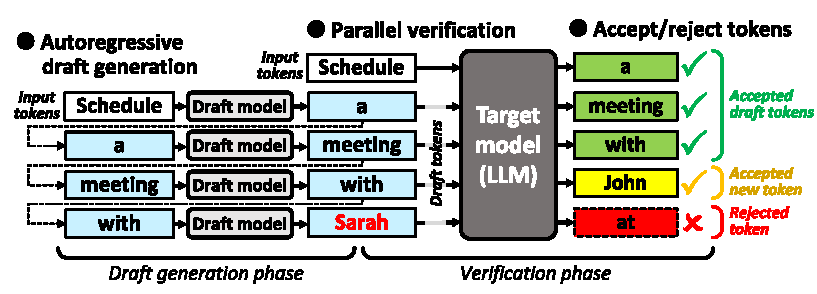
\includegraphics[width=\columnwidth]{./fig/specdec}
\caption{
Illustration of speculative decoding.
}
\Description{Illustration of speculative decoding.}
\label{fig:specdec}
\end{figure}


\begin{figure}[t!] \centering
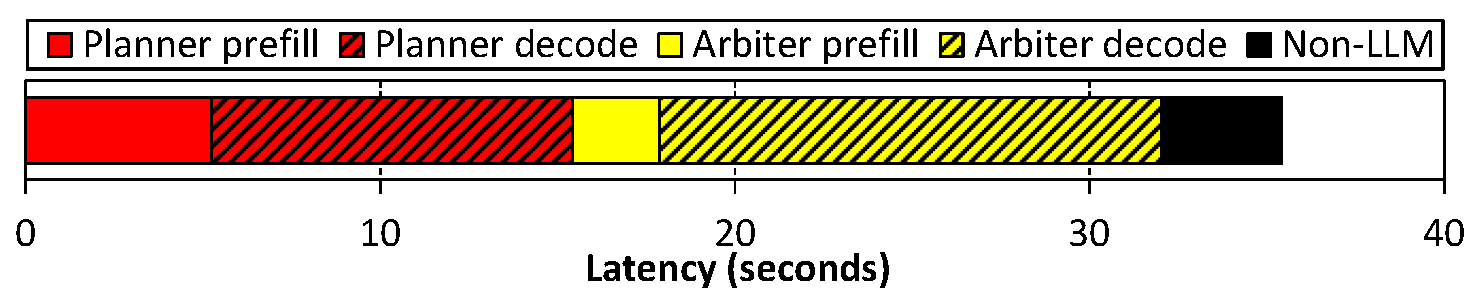
\includegraphics[width=\columnwidth]{./fig/agent_breakdown_latency}
\caption{
Latency breakdown of agentic tasks.
}
\Description{Latency breakdown of agentic tasks.}
\label{fig:agent_breakdown_latency}
\end{figure}

\fig{fig:agent_breakdown_latency} breaks down the end-to-end latency of agentic task executions. The two LLM components, Planner (43.5\%) and Arbiter (46.9\%), together account for 90.4\% of the total latency. Notably, while decode dominates (68.7\%), the prefill stage remains a significant contributor (21.7\%). This contrasts with conventional LLM workloads executed in the cloud using server-class devices, where decode latency is overwhelmingly dominant (e.g., over 95\%, 98\%, and 98\% in WSC-LLM~\cite{wsc_llm}, FDC~\cite{fdc}, and CENT~\cite{cent}), rendering the LLM decode stage the primary bottleneck to address.

We identify two main reasons for the differing bottlenecks between conventional LLMs and agentic workloads. First, prior work~\cite{gemini_2.5} reports that agents typically process much longer input token sequences than they generate as output, a trend we confirmed in our own measurements. This imbalance makes the LLM prefill stage of agents far more compute‑intensive than in conventional LLMs. Second, the cost of processing these longer inputs is magnified by limited hardware resources of today’s on‑device accelerators, rendering prefill disproportionately expensive. \tab{tab:server_vs_edge_chips} compares modern AI chips and reveals that on‑device accelerators provide at most 11\% of the memory bandwidth and roughly 2\% of the compute throughput of server‑class NVIDIA H200 GPU~\cite{nvidia_h200_sxm}. Together, these factors make the compute‑bound prefill more expensive than decode, leaving \emph{both} stages as two dominant performance bottlenecks in AI agents.

Overall, because the compute‑bound prefill and memory bandwidth‑bound decode phases now contribute comparable amounts of latency, no single stage or model instance dominates. Effective acceleration of agentic systems must therefore optimize the \textit{entire} Planner–Arbiter pipeline, improving both prefill and decode. In the remainder of this section, we present a token‑level characterization of the Planner and Arbiter prefill and decode stages that motivates our proposed \prefill and \decode.


\begin{table}[t!]
\centering
\caption{
The compute throughput and memory bandwidth available in modern AI chips, both high-end server-class devices and on-device accelerators.
}
\scriptsize
\begin{tabular}{|c|c|c|c|}
\hline
\textbf{Device} & \textbf{Class} & \makecell[c]{\textbf{Compute power}\\ \textbf{(INT8 TOPS)}} & \makecell[c]{\textbf{Memory}\\ \textbf{bandwidth (GB/s)}} \\
\hline
\textbf{NVIDIA H100}~\cite{nvidia_h100_sxm} & \multirow{5}{*}{\centering Server} & 1,979 & 3,350 \\
\cline{1-1} \cline{3-4}
\textbf{NVIDIA H200}~\cite{nvidia_h200_sxm} & & 1,979 & 4,800 \\
\cline{1-1} \cline{3-4}
\textbf{NVIDIA B200}~\cite{nvidia_b200_sxm} & & 4,500 & 8,000 \\
\cline{1-1} \cline{3-4}
\textbf{AMD MI325X}~\cite{amd_mi325x} & & 2,615 & 6,000 \\
\cline{1-1} \cline{3-4}
\textbf{Google TPU v6e}~\cite{google_tpu_v6e} & & 1,836 & 1,640 \\
\hline
\textbf{Apple M4 Max}~\cite{apple_m4_pro_max} & \multirow{5}{*}{\centering On-device} & 38 & 546 \\
\cline{1-1} \cline{3-4}
\makecell[c]{\textbf{Qualcomm Snapdragon}\\ \textbf{X Elite}~\cite{qualcomm_snapdragon_x_elite}} &  & 45 & 135 \\
\cline{1-1} \cline{3-4}
\makecell[c]{\textbf{AMD Ryzen}\\ \textbf{AI+ PRO 395}~\cite{amd_ryzen_ai_max}} &  & 50 & 256 \\
\hline
\end{tabular}
\label{tab:server_vs_edge_chips}
\end{table}


\begin{figure}[t!] \centering
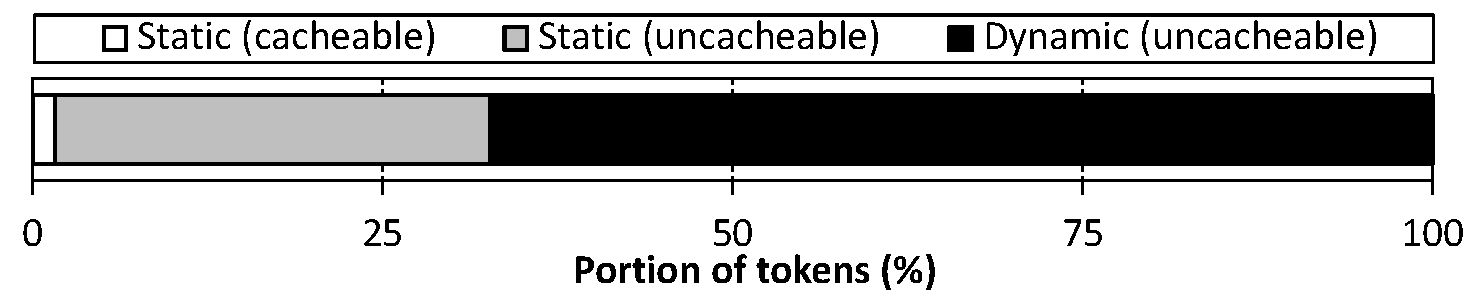
\includegraphics[width=\columnwidth]{./fig/agent_breakdown_token}
\caption{
Token count breakdown of Planner inputs. Results are averaged across all examples in the TinyAgent fine-tuning test dataset. Static tokens are uncacheable if they are placed behind dynamic tokens.
}
\Description{Token count breakdown of Planner inputs.}
\label{fig:agent_breakdown_token}
\end{figure}


\subsection{Prefill Stage Token Analysis} \label{sect:prefill_analysis}

{\bf Planner input tokens.} The Planner input consists of the static system prompt, retrieved tool descriptions and guidelines, and retrieved tool-use examples (see \fig{fig:plan-out_agents}). \fig{fig:agent_breakdown_token} shows the average token-count distribution of Planner inputs. Out of the total 1,739 tokens, the static system prompt takes up 32.7\%, suggesting that prefix caching could potentially accelerate prefill. However, because the dynamically retrieved tool descriptions and guidelines are inserted into the Planner input early on, the first dynamic token appears after only 1.6\% of the prompt, limiting KV cache reuse if the input prompts are used as-is (see \fig{fig:prefix_caching}). Encouragingly, we observe that the dynamically changing tool descriptions and guidelines are different combinations of static fragments, where the combinations depend solely on the selected tool sets. If the tool descriptions and guidelines were made static, the number of uncacheable tokens would decrease by 32\% (1,711 to 1,171). \textit{Overall, the potential of prefix caching is hindered by early dynamicity introduced by tool descriptions and guidelines, which are merely rearranged chunks of static prompts.}


\begin{figure}[t!] \centering
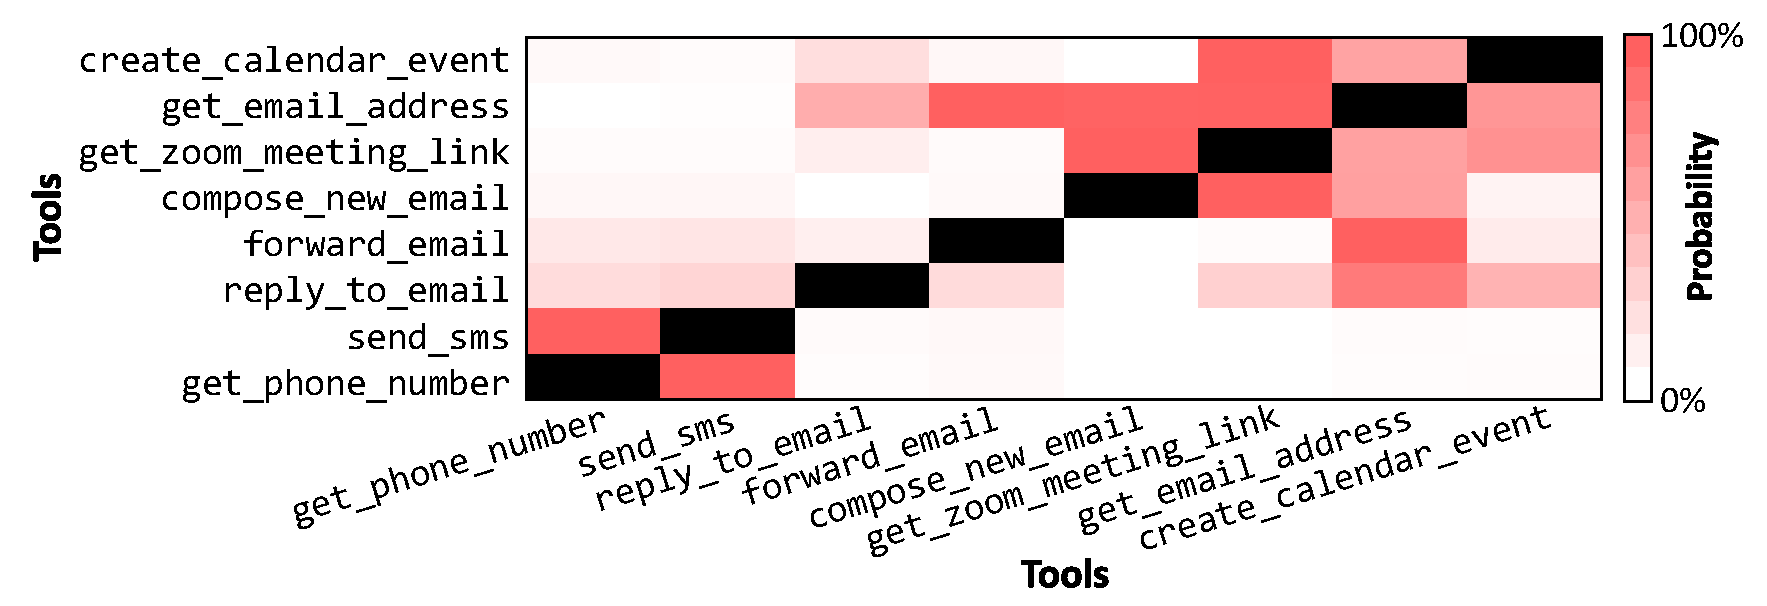
\includegraphics[width=\columnwidth]{./fig/tool_heatmap}
\caption{
Tool co-activation heatmap of a subset of tools in TinyAgent training dataset. The value at $(x,y)$ depicts how likely $\text{tool}_y$ is to be activated given that $\text{tool}_x$ has been activated, i.e., $P(\text{tool}_y | \text{tool}_x)$.
}
\Description{Tool co-activation heatmap of a subset of tools in TinyAgent training dataset.}
\label{fig:tool_heatmap}
\end{figure}


We also observe the existence of \textit{tool co-activation locality} in the Planner's input prompts, which we define as the likelihood of certain tools being called together across different queries. This skewness in tool co-activation is illustrated in \fig{fig:tool_heatmap} as a heatmap. For example, \texttt{get\_zoom\_meeting\_link} is more likely to be co-activated with \texttt{get\_email\_address} (91\%) or \texttt{compose\_new\_email} (58\%) than \texttt{get\_phone\_number} (6\%). This is because the nature of agentic tasks suggests that tools which fall under the same theme (e.g., email, contacts, maps, and notes) are more likely to be retrieved together in the same plan. This locality is further extended to inter-theme relations, where certain themes like contact and email are ``closer'' in their relationship than others such as contact and maps. \textit{Thus, our characterization reveals that tool co‑activation locality is intrinsic to agentic applications.}

In the tool-use example retrieval process, the top-$K$ examples displaying the most similar text embedding to the current user query are retrieved (\sect{sect:on_device_agents}). While users typically query tasks requiring the use of multiple tools (82\% of TinyAgent training dataset), we observe that single-tool examples are retrieved as relevant examples 57\% of the time. In other words, \textit{the single-tool examples are important as tool-use examples for planning tasks.} This is not to be confused with the existence of tool co-activation locality in the choice of tools, as the dominance of single-tool examples is observed in the choice of tool-use examples.


{\bf Arbiter input tokens.} The Arbiter’s input includes decision guidelines and examples, along with the list of call-observation pairs produced by tool execution (see \fig{fig:plan-out_agents}). Depending on the internal LLMCompiler state, only two static prefix variants occur; these prefixes account for 88\% and 90\% of the Arbiter input, respectively. \textit{Because the Arbiter input contains such a large static prefix, prefix caching can capture it effectively.}

\subsection{Decode Stage Token Analysis} \label{sect:decode_analysis}

\begin{figure}[t!] \centering
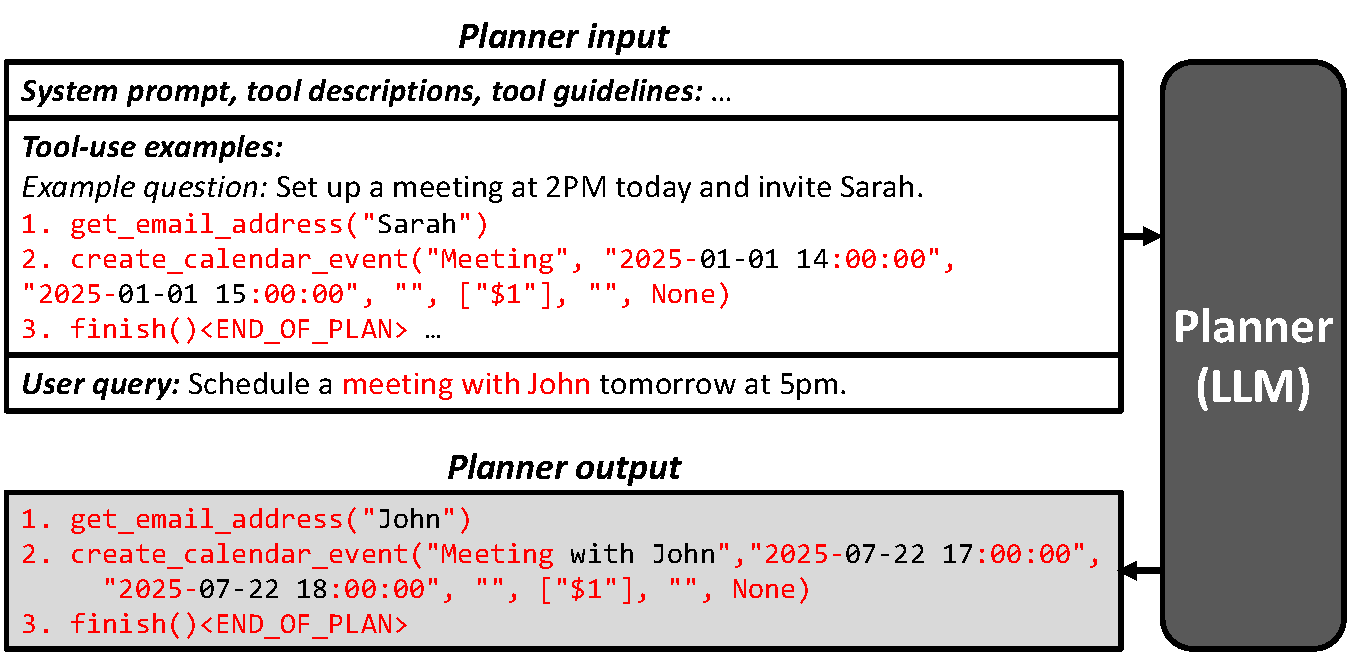
\includegraphics[width=\columnwidth]{./fig/planner_token_example}
\caption{
Input and output example of Planner for the query \textit{``Schedule a meeting with John tomorrow at 5pm.''}
}
\Description{Input and output example of Planner for the query ``Schedule a meeting with John tomorrow at 5pm.''}
\label{fig:planner_token_example}
\end{figure}


{\bf Planner and Arbiter output tokens.} \fig{fig:planner_token_example} shows an example tool-use example alongside the output for the query \textit{``Schedule a meeting with John tomorrow at 5pm.''} The generated plans share the same structural template as the tool-use example, with arguments substituted to match the user query. This occurs because the tool names, their arguments, and tool-calling orders are mostly embedded in the tool-use examples. Empirically, 96\% of Planner and 87\% of Arbiter output tokens overlap with those in their corresponding input prompt. \textit{Overall, our key observation is that the output tokens generated in both Planner and Arbiter's decode stage are highly correlated with provided examples and user prompt.}

While their outputs display highly regular and predictable patterns, reflecting the templates provided by the few-shot examples in the prompt, the decode stages of Planner and Arbiter account for 68.7\% of the end-to-end latency. Therefore, we conclude that \textit{the decode stage of agentic LLMs is inefficient in that a large portion of time is spent generating straightforward, formulaic sequences that do not require the reasoning capabilities of LLMs.}


{\bf Challenges of applying speculative decoding.} Despite its promise, speculative decoding requires a carefully chosen draft model for high efficiency, and selecting one is nontrivial. If the draft model is too small, it fails to produce high‑quality draft tokens and yields little performance improvement. Conversely, a larger draft model achieves higher token accuracy (i.e., the fraction of draft tokens ultimately accepted during verification) but introduces substantial latency overhead.

The \textit{Theoretical~max.~speedup} column of \tab{tab:draft_specdec_accuracy} reports the maximum speedup achievable by each draft model under the Planner workload. We compute this theoretical limit analytically, assuming that the LLM decode stage is memory bandwidth‑limited and that its latency therefore scales proportionally with model size. Leveraging this assumption, we combine the draft‑token accuracy (second column of \tab{tab:draft_specdec_accuracy}) to estimate the final output‑token count and its corresponding latency, which we then compare with the baseline to derive the projected speedup. As shown, even with state-of-the-art small LLMs~\cite{llama_3.2} or fine-tuned draft models from prior work~\cite{specinfer}, it is difficult to balance the accuracy and draft model size, where smaller draft LLMs barely yield any speedup due to their low draft token accuracy while large draft LLMs with high draft token latency end up spending too much time generating draft tokens.


\begin{table}[t]
\centering
\caption{
Draft token accuracy and achievable theoretical speedups of various draft models.
}
\footnotesize
\resizebox{1.0\columnwidth}{!}{
\begin{tabular}{|c|c|c|c|}
\hline
\textbf{Draft model} & \makecell[c]{\textbf{Draft token}\\ \textbf{accuracy}} & \makecell[c]{\textbf{Theoretical}\\ \textbf{max. speedup}} & \makecell[c]{\textbf{Speedup}\\ \textbf{(with tax)}} \\
\hline
\textbf{Llama-3.2-3B-Instruct} & 0.42 & 0.96$\times$ & 0.83$\times$ \\
\hline
\textbf{Llama-3.2-1B-Instruct} & 0.33 & 1.59$\times$ & 1.20$\times$ \\
\hline
\textbf{Llama-160M} & 0.02 & 0.98$\times$ & 0.57$\times$ \\
\hline
\textbf{Llama-68M} & 0.02 & 1.11$\times$ & 0.62$\times$ \\
\hline
\end{tabular}
}
\label{tab:draft_specdec_accuracy}
\end{table}


\begin{figure}[t!] \centering
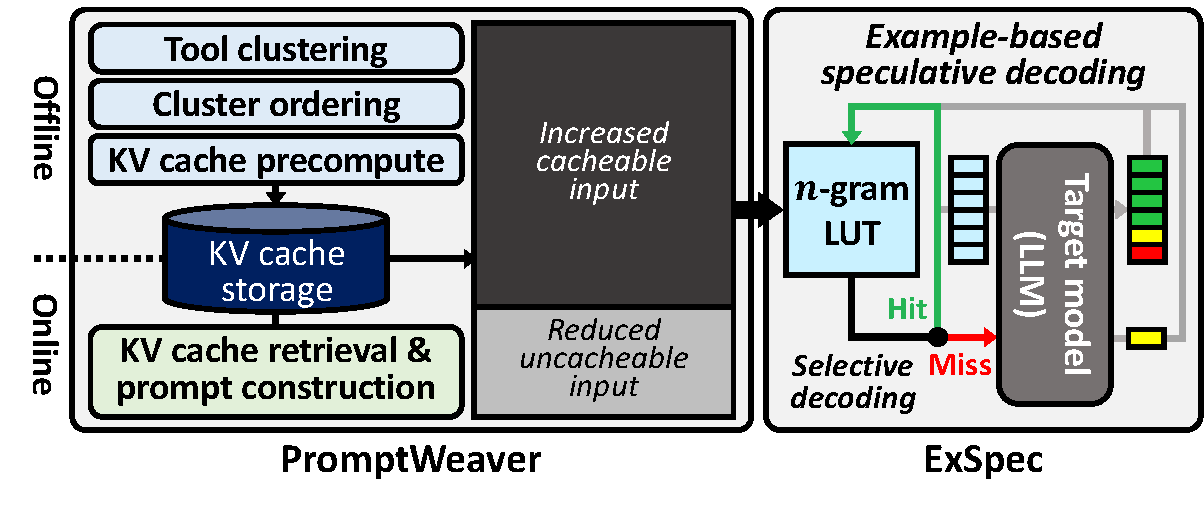
\includegraphics[width=\columnwidth]{./fig/proposed_overview}
\caption{
Proposed \proposed system architecture. 
}
\Description{Proposed \proposed system architecture. }
\label{fig:proposed_overview}
\end{figure}


Now, recall from \fig{fig:specdec} that speculative decoding requires both single‑token inference by the draft LLM (autoregressive token generation) and multi‑token inference by the target LLM (parallel verification). However, on-device AI systems are increasingly being optimized for single-batch LLM calls~\cite{decdec, llm_in_a_flash, cambricon_llm, edgemoe, edgellm}. For example, in Apple's official LLM framework MLX-LM~\cite{mlx_lm}, a single-token autoregressive inference with TinyAgent takes 131 ms per token, while the same model's verification phase with 2 tokens takes 244 ms, resulting in a 1.86$\times$ slowdown. This phenomenon, which we refer to as \textit{the multi-token tax}, degrades the overall performance of on-device speculative decoding schemes, where multiple tokens must be verified by the target LLM. Based on this slowdown, we recompute the speedup of applying speculative decoding in the \textit{Speedup~(with~tax)} column of \tab{tab:draft_specdec_accuracy}. The best achievable speedup among state-of-the-art small LLMs~\cite{llama_3.2} or draft LLMs fine-tuned by prior work~\cite{specinfer} is 1.20$\times$. \textit{Therefore, we conclude that applying speculative decoding to on-device frameworks is challenging due to the multi-token tax and draft LLM latency overhead.}